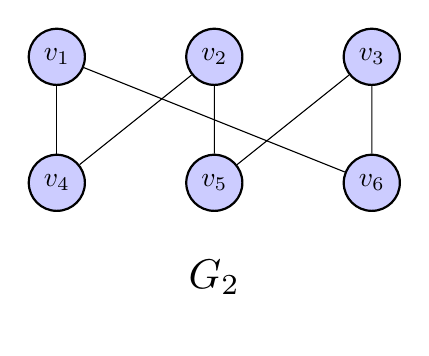
\begin{tikzpicture}
  [scale=.8,auto=left,every node/.style={circle,fill=blue!20,draw=black,thick}]
  
  % Fila superior (equivalente a la columna izquierda original)
  \node (n1) at (0,2) {$v_1$};
  \node (n2) at (2.5,2) {$v_2$};
  \node (n3) at (5,2) {$v_3$};

  % Fila inferior (equivalente a la columna derecha original)
  \node (n4) at (0,0) {$v_4$};
  \node (n5) at (2.5,0) {$v_5$};
  \node (n6) at (5,0) {$v_6$};

  % Aristas correspondientes a la imagen original
  \foreach \from/\to in {n1/n4, n1/n6, n2/n4, n2/n5, n3/n5, n3/n6}
    \draw (\from) -- (\to);

  % Etiqueta G_2 debajo del grafo
  \node[draw=none, fill=none, scale=1.5] at (2.5,-1.5) {$G_2$};

\end{tikzpicture}
